\documentclass[12pt]{article}
\usepackage{amsmath}
\usepackage{graphicx}

\title{Reference Angles}
\author{Zach Latta}
\date{0.8.29.13}

\newcommand{\degree}{\ensuremath{^\circ}}

\begin{document}

\maketitle

A reference angle is an angle created by the terminal side and the x-axis.

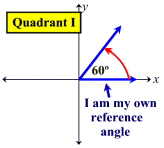
\includegraphics{assets/reference_angle_1.png}
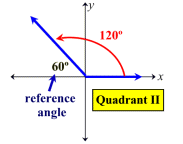
\includegraphics{assets/reference_angle_2.png}
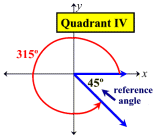
\includegraphics{assets/reference_angle_4.png}
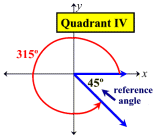
\includegraphics{assets/reference_angle_4.png}

\end{document}
